\documentclass{beamer}
\usepackage[utf8]{inputenc}
\usepackage{adjustbox}
\usepackage{array,ragged2e}
\usepackage{longtable}
\usepackage{pdflscape}
\usepackage{makecell}
\usepackage[font=tiny]{caption}
\usepackage{booktabs}
\usepackage[capposition=bottom]{floatrow}

\usepackage{amssymb}
\usepackage{amsfonts}
\usepackage{amsthm}
\usepackage{amsmath}
\usepackage{amsmath,systeme}
\usepackage{spalign}
\usepackage{tikz}
\usepackage{nicematrix}
\usepackage{float}
\usepackage{lmodern}
\usepackage{graphicx}
\usetikzlibrary{tikzmark}
\usetikzlibrary{arrows.meta}
\usepackage{wasysym}
\usepackage{fontawesome}

\floatstyle{plaintop}
\restylefloat{table}
\usepackage[edges]{forest}

% Grey Box Hightlight
\usepackage{tcolorbox}

% Fancy table
\usepackage{tcolorbox}
\usepackage{tabularx}
\usepackage{array}
\usepackage{colortbl}
\tcbuselibrary{skins}

\newcolumntype{Y}{>{\raggedleft\arraybackslash}X}


% Code Listing Settings
\usepackage{listings}
\lstset{
	language=Python,
	basicstyle=\ttfamily,
	aboveskip={1.0\baselineskip},
	belowskip={1.0\baselineskip},
	columns=fixed,
	extendedchars=true,
	breaklines=true,
	tabsize=4,
	prebreak=\raisebox{0ex}[0ex][0ex]{\ensuremath{\hookleftarrow}},
	frame=lines,
	showtabs=false,
	showspaces=false,
	showstringspaces=false,
	keywordstyle=\color[rgb]{0.627,0.126,0.941},
	commentstyle=\color[rgb]{0.133,0.545,0.133},
	stringstyle=\color[rgb]{01,0,0},
	numbers=left,
	stepnumber=1,
	numbersep=10pt,
	captionpos=t,
	escapeinside={\%*}{*)}
}

\newcommand{\subf}[2]{%
	{\small \begin{tabular}[t]{@{}c@{}}
			\mbox{}\\[-\ht\strutbox]
			#1\\#2
	\end{tabular}}%
}

\usetheme{Madrid}
\usecolortheme{default}
\useinnertheme{circles}

\setbeamertemplate{footline}[text line]{%
	\parbox{\linewidth}{\hfill\insertpagenumber}}
\setbeamertemplate{navigation symbols}{}

\setbeamertemplate{caption}[numbered]

\definecolor{UCLAblue}{RGB}{39, 116, 174}
\definecolor{UCLAgold}{RGB}{255, 209, 0}

\setbeamercolor*{palette primary}{bg=UCLAblue, fg=UCLAgold}
\setbeamercolor*{palette secondary}{bg=white, fg=black}
\setbeamercolor*{palette tertiary}{bg=white, fg=black}
\setbeamercolor*{palette quaternary}{bg=white,fg=black}
\setbeamercolor{structure}{fg=UCLAblue} % itemize, enumerate, etc
\setbeamercolor{section in toc}{fg=UCLAblue} % TOC sections

\tcbset{tab2/.style={enhanced,fonttitle=\bfseries,fontupper=\footnotesize,
		colback=yellow!10!white,colframe=UCLAblue,colbacktitle=yellow!10!white,
		coltitle=black,center title}}
	
\def\Arrow{\raisebox{-.5\height}{\scalebox{4}{$\Rightarrow$}}}

% For cross-validation visualization
\newcommand*\revealcline{\noalign{\vskip\arrayrulewidth}}
\newcommand*\nextrow[1]
{\\\cline{#1}\noalign{\vskip1ex}\cline{#1}\revealcline}
\newcount\ccellA
\newcommand*\ccellOut[2]
{%
	\def\tmpa{}%
	\ccellA=1
	\loop
	\ifnum#1=\ccellA
	\edef\tmpa{\unexpanded\expandafter{\tmpa\cellcolor{UCLAblue}}}%
	\fi
	\ifnum#2>\ccellA
	\advance\ccellA1
	\edef\tmpa{\unexpanded\expandafter{\tmpa&}}%
	\repeat
	\tmpa
}


\newcommand*\ccellIn[2]
{%
	\def\tmpa{}%
	\ccellA=1
	\loop
	\ifnum#1=\ccellA
	\edef\tmpa{\unexpanded\expandafter{\tmpa\cellcolor{UCLAgold}}}%
	\fi
	\ifnum#2>\ccellA
	\advance\ccellA1
	\edef\tmpa{\unexpanded\expandafter{\tmpa&}}%
	\repeat
	\tmpa
}


\graphicspath{{/Users/zionsheng/Desktop/Duke/23fa/ECE899/week1/img}}

% \let\footnoterule\relax
\renewcommand{\footnoterule}{%
	\kern 0.1mm
	\hrule width \textwidth height 0.8pt
	\kern 1mm
}

\newtcbox{\mybox}[1][red]{on line,
	colback=#1, colframe=#1, boxsep=0pt, boxrule=0pt, size=small, arc=1mm}

\usepackage{hyperref}
\hypersetup{colorlinks=true,
	linkcolor=blue,
	filecolor=magenta,      
	urlcolor=cyan}

\tikzset{
	point/.style = {% define a style for the function points
		circle,
		fill=#1,
		draw=black,
		inner sep=2pt,
	},
	point/.default = {violet!60}
}

\AtBeginSection[]{
	\begin{frame}
		\vfill
		\centering
		\begin{beamercolorbox}[sep=8pt,center,shadow=true,rounded=true]{title}
			\usebeamerfont{title}\insertsectionhead\par%
		\end{beamercolorbox}
		\vfill
	\end{frame}
}

%-------------------------------------------------------------------------------
% This block of code defines the information to appear in the Title page
\title[Independent Study Weekly Meeting 1] %optional
{Independent Study Weekly Meeting 1}

\subtitle{A quick review of the two journal papers I read (Part 1/2)}

\author[Zion Sheng] % (optional)
{Zion Sheng}

\institute[Duke ECE] % (optional)
{
	Department of ECE\\
	Duke University
}

\begin{document}
	\justifying
	\frame{\titlepage} 

	\begin{frame}
		\frametitle{Table of Contents}
		\tableofcontents
	\end{frame}

	\section{Part 1. The Current Progress}
	\begin{frame}[t]
		\frametitle{The Current Progress}
		\textbf{Completed}
		\begin{itemize}
			\justifying
			\item Read through Paper 1 but skipped some details in the result analysis section temperorily.
			\item Read the section 1 (Introduction), section 2 (Adaptive Stimulus Selection Algorithm) and section 5 (Conclusion)
			\item Started to go through a \texttt{MNE} instruction (\href{https://www.youtube.com/watch?v=t-twhNqgfSY&t=439s}{Videos} and \href{https://github.com/zs144/learn-pybrain-mne}{Jyputer Notebook}), but paused it due to the steady progress on paper reading.
		\end{itemize}

		\textbf{Doing}
			\begin{itemize}
				\justifying
				\item Trying to understand the model more throughoutly.
				\item Reading Paper 3 (Mainsah et al, 2016) to figure out how to run the simulation and online experiment conducted in Paper 2.
			\end{itemize}

	\end{frame}
	
	\section{Part 2. Review on Paper 1 (Farwell and Donchin, 1988)}
	\begin{frame}[t]
		\frametitle{Review on Paper 1}
		\begin{minipage}{0.4\linewidth}
			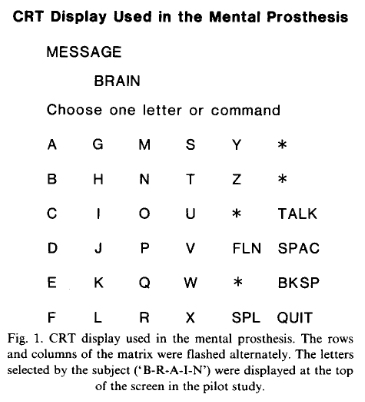
\includegraphics[width=5cm]{screen_display.jpg}
		\end{minipage}
		\vspace{3mm}
		\hspace{1mm}
		\begin{minipage}{0.55\linewidth}
			\scriptsize
			This paper describes the development and testing of a system whereby one can communicate through a computer by using the P300 component of the event-related brain potential (ERP). Such a system may be used as a communication aid by individuals who cannot use any motor system for communication (e.g., 'locked-in' patients). The 26 letters of the alphabet, together with several other symbols and commands, are displayed on a computer screen which serves as the keyboard or prosthetic device. The subject focuses attention successively on the characters he wishes to communicate. The computer detects the chosen character on-line and in real time. This detection is achieved by repeatedly flashing rows and columns of the matrix. When the elements containing the chosen character are flashed, a P300 is elicited, and it is this P300 that is detected by the computer. \\
		\end{minipage}
	
		\scriptsize
		The paper tries to estimate the smallest number of trials that must be used to reduce the signal-to-noise level in the ERP signal so that the character the subject has chosen could be communicated at a specified level of certainty. However, the speed is rather slow for this first version of P300 speller, which is about 2.3 characters/minute. What about some latest ones?
	\end{frame}
	
	\section{Part 3. Review on Paper 2 (Mainsah et al, 2017)}
	\begin{frame}[t]
		\frametitle{Review on Paper 2}
		The paper derives a simple analytical solution of an information-based objective function for BCI stimulus selection by transforming the high-dimensional stimulus space into a one-dimensional space that parameterizes the objective function - the prior probability mass of the stimulus under consideration, irrespective of its contents. 
		\begin{itemize}
			\justifying
			\item Previous stimulus paradigms do not necessarily provide the best approach to maximize BCI performance as not every stimulus provides the same amount of utility to estimate the user's intent based on the currently observed data.
			\item The objective function is now conveniently parameterized by P 1t, the total prior probability of characters within a flash group.
		\end{itemize}
		
	\end{frame}

	\section{Part 4. Summary}


	
	\section{Part 5. Get Ready for the Next Step}
		
	
\end{document}